\section{Problemas de Optimización}

\subsection*{Procedimiento}
El problema se plantea por lo general como el cálculo del máximo o del mínimo de una función de varias variables y nos proporcionan ecuaciones de ``ligadura'' entre las variables gracias a las cuales terminamos buscando los máximos y los mínimos de una función de una variable\footnote{Cuando estudiemos cálculo en varias variables veremos otros métodos.}. 

\subsection*{Trucos}
\begin{enumerate}
    \item El máximo o el mínimo de $f(x)$ se alcanza en los mismos puntos que lo alcanza la función $g(x)=kf(x)$, con $k>0$.

    \item Si $g$ es estrictamente creciente, entonces los máximos y los mínimos absolutos de $f(x)$ y $h(x)=g(f(x))$ se alcanzan en los mismos puntos.
    \begin{proof}
    Demostramos para el mínimo, ya que para el máximo es análoga.
    
        Supongamos $a$ mínimo de $f \Longrightarrow f(a) \leq f(x)\;\forall x\in I$.

        Como $g$ es estrictamente creciente, $g(f(a)) \leq g(f(x))\; \forall x\in I$.
    \end{proof}

    \item $f(x)$ y $f^2(x)$ alcanzan los máximos y los mínimos en los mismos puntos si $f(x)\geq 0\quad \forall x$, ya que $f^2(x)=g(f(x))$, con $g(x)=x^2$ y $g$ es estrictamente creciente en $\bb{R}^+_0$.

    \item $f(x)$ y $e^{f(x)}$ alcanzan los máximos y los mínimos en los mismos puntos.
\end{enumerate}

\begin{ejercicio}
    Una caja abierta está construida con un rectángulo de cartón, quitando cuadrados iguales en cada esquina y doblando hacia arriba los bordes. Hállense las dimensiones de la caja de mayor volumen que puede construirse con ese procedimiento si el rectángulo tiene como lados:
    \begin{enumerate}
        \item 10 y 10
        \begin{figure}[H]
            \centering
            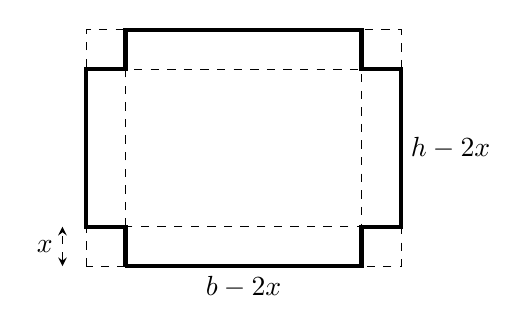
\begin{tikzpicture}
                \def\b{4}
                \def\h{3}
                \def\x{0.5}
                \draw[dashed] (0,0) rectangle (\b,\h);
                \draw[dashed] (\x,\x) rectangle (\b-\x,\h-\x);

                \draw[ultra thick] (\x,0) -- (\b-\x,0) -- (\b-\x, \x) -- (\b-\x, \x) -- (\b, \x) -- (\b,\h-\x) -- (\b-\x, \h-\x) -- (\b-\x, \h) -- (\x,\h) -- (\x, \h-\x) -- (0, \h-\x) -- (0, \x) -- (\x, \x) -- (\x, 0);

                \node at (\b/2, 0)[below]  {$b-2x$};
                \node at (\b, \h/2)[right]  {$h-2x$};

                \draw [stealth-stealth, dashed] (-0.3,0) -- node[left]{$x$} (-0.3, \x);
            \end{tikzpicture}
        \end{figure}
        Trabajamos de forma general con los valores de altura $h$ y base $b$ como constantes. La medida $x$ es el lado del cuadrado que se ha recortado. El volumen de la caja será:
        \begin{equation*}
            \begin{array}{rl}
                V:\left]0, \frac{\min(b,h)}{2}\right[ & \longrightarrow \bb{R}\\
                        x & \longmapsto V(x) = x(b-2x)(h-2x) = bhx-2x^2(b+h)+4x^3
            \end{array}
        \end{equation*}
        Para maximizar el volumen de la caja, le hallamos los extremos relativos a la función $V$:
        \begin{equation*}
            V'(x)=bh - 4(b+h)x + 12x^2
        \end{equation*}
        Para $b=h=10\;u$, los puntos críticos son:
        \begin{equation*}
            V'(x)=0\Longrightarrow 12x^2 - 80x + 100 = 0 \Longrightarrow 3x^2 - 20x + 25=0\Longrightarrow  \left\{\begin{array}{l}
                x = \frac{5}{3}\;u \\
                \xcancel{x=5}
            \end{array}\right.
        \end{equation*}

        Veamos si, efectivamente, los puntos críticos son extremos relativos:
        \begin{itemize}
            \item \underline{Para $x<\frac{5}{3}$} $V'(x)>0 \Longrightarrow V$ estrictamente creciente.
            \item \underline{Para $x>\frac{5}{3}$} $V'(x)<0 \Longrightarrow V$ estrictamente decreciente.

        Por tanto, efectivamente obtenemos un máximo relativo en $x=\frac{5}{3}\;u.$ El volumen para estas dimensiones es $V=\frac{2000}{27}\approx 74.074\;u^3$.

        Además, efectivamente obtenemos un máximo absoluto, ya que
        $$\lim_{x\to 0^+}V(x) = \lim_{x\to 5^-}V(x) = 0 < V\left(\frac{5}{3}\right) = \frac{2000}{27}\;u^3$$

        Por tanto, las dimensiones pedidas son:
        $$x=\frac{5}{3}\;u \qquad V=\frac{2000}{27}\approx 74.074\;u^3$$
        \end{itemize}
        
        \item 12 y 18\\
        Siguiendo un razonamiento análogo, para $b=12$ y $h=18\;u$, los puntos críticos son:
        \begin{equation*}
            V'(x)=0\Longrightarrow 12x^2 - 120x + 216 = 0 \Longrightarrow x^2 - 10x + 18=0\Longrightarrow  \left\{\begin{array}{l}
                x = 5-\sqrt{7}\;u \\
                \xcancel{x=5+\sqrt{7}}
            \end{array}\right.
        \end{equation*}

        Veamos si, efectivamente, los puntos críticos son extremos relativos:
        \begin{itemize}
            \item \underline{Para $x<5-\sqrt{7}$} $V'(x)>0 \Longrightarrow V$ estrictamente creciente.
            \item \underline{Para $x>5-\sqrt{7}$} $V'(x)<0 \Longrightarrow V$ estrictamente decreciente.

        Por tanto, efectivamente obtenemos un máximo relativo en $x=5-\sqrt{7}\;u.$ El volumen para estas dimensiones es $V=V(5-\sqrt{7})\approx 228.162\;u^3$.

        Además, efectivamente obtenemos un máximo absoluto, ya que
        $$\lim_{x\to 0^+}V(x) = \lim_{x\to 6^-}V(x) = 0 < V\left(5-\sqrt{7}\right) \approx 228.162\;u^3$$

        Por tanto, las dimensiones pedidas son:
        $$x=5-\sqrt{7}\;u \qquad V\approx 228.162\;u^3$$
        \end{itemize}
    \end{enumerate}
\end{ejercicio}

\begin{ejercicio}
    Se desea construir una ventana con forma de rectángulo coronado de un semicírculo de diámetro igual a la base del rectángulo. Pondremos cristal blanco en la parte rectangular y cristal de color en el semicírculo. Sabiendo que el cristal coloreado deja pasar la mitad de luz (por unidad de superficie) que el blanco, calcúlense las dimensiones de la ventana para conseguir la máxima luminosidad si se ha de mantener un perímetro constante dado.
    \begin{figure}[H]
        \centering
        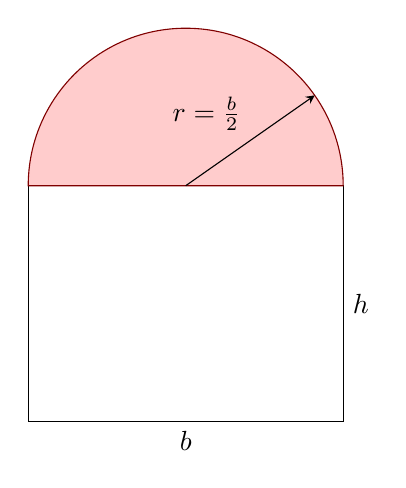
\begin{tikzpicture}
            \def\b{4}
            \def\h{3}
            \draw(0,0) rectangle (\b,\h);
            \filldraw[fill=red!20!white, draw=red!50!black] (0,\h) arc (180:0:\b/2) -- cycle;
            
            \node at (\b/2, 0)[below]  {$b$};
            \node at (\b, \h/2)[right]  {$h$};

            \def\ang{35}
            \pgfmathsetmacro{\x}{\b/2 + (\b/2)*cos(\ang)};
            \pgfmathsetmacro{\y}{\h +  (\b/2)*sin(\ang)};
            \draw[-stealth] (\b/2, \h) -- node[above left]{$r=\frac{b}{2}$} (\x,\y);
        \end{tikzpicture}
    \end{figure}

    La ecuación de ligadura dada es que el perímetro es constante, es decir:
    $$P=b+2h+\frac{2\pi r}{2} = b+2h+\pi r = b+2h + \frac{\pi b}{2} \Longrightarrow h = \frac{P-b(1+\frac{\pi}{2})}{2}$$

    La ecuación a maximizar $L$ que indica la luminosidad obtenida es:
    \begin{equation*}
        \begin{array}{rl}
            L:\bb{R}^+ & \longrightarrow \bb{R}\\
                    b & \longmapsto L(b) = A_B + \frac{A_R}{2} = bh +  \frac{1}{2} \frac{\pi \frac{b^2}{4}}{2}
                    = \frac{Pb-b^2(1+\frac{\pi}{2})}{2} + \frac{\pi b^2}{16} 
        \end{array}
    \end{equation*}

    Para maximizarla, le hallo los extremos relativos:
    \begin{equation*}
        L'(b) = \frac{P}{2} - b\left(1+\frac{\pi}{2}\right) + \frac{\pi b}{8}
    \end{equation*}
    por tanto,
    \begin{equation*}
        L'(b) = 0 \Longleftrightarrow b\left(1+\frac{\pi}{2} - \frac{\pi}{8}\right) = \frac{P}{2} \Longleftrightarrow b = \frac{P}{2\left(1+\frac{3\pi}{8}\right)} = \frac{P}{2+\frac{3\pi}{4}} = \frac{4 P}{8+3\pi}
    \end{equation*}

    Comprobemos si, efectivamente, el punto crítico es un extremo relativo.
    \begin{equation*}
        L''(b) = -1 - \frac{\pi}{2} + \frac{\pi}{8} < 0 \quad \forall b \in \bb{R}^+
    \end{equation*}

    Por tanto, como $L''\left(\frac{4 P}{8+3\pi} \right) < 0 \Longrightarrow b = \frac{4 P}{8+3\pi}$ es un máximo relativo. Además, es máximo absoluto ya que $L(b)$ es continua y solo tiene un extremo relativo. Por tanto, las dimensiones son:
    \begin{gather*}
        h = \frac{P-\frac{4 P}{8+3\pi}\left(1+\frac{\pi}{2}\right)}{2}
        =\frac{P-\frac{4 P}{8+3\pi}-\frac{2 P\pi}{8+3\pi}}{2}
        = P\frac{8+3\pi-4-2\pi}{2(8+3\pi)}
        = P\frac{4+\pi}{2(8+3\pi)}\\
        b=\frac{4 P}{8+3\pi} \qquad r=\frac{b}{2} = \frac{2P}{8+3\pi}
    \end{gather*}
    
\end{ejercicio}

\begin{ejercicio}
    Las palomas domésticas no suelen volar sobre extensiones grandes de agua a menos que se vean forzadas a ello, posiblemente porque se requiera más energía para mantener la altitud sobre el agua fría. Supongamos que se suelta una paloma desde un barco situado a 3 km de la costa, siendo $A$ el punto costero más cercano. El palomar se encuentra en un punto de la costa situado a 10 km de $A$. Si la paloma gasta dos veces más energía volando sobre el agua que sobre la tierra firme y sigue un camino que hace mínima la energía gastada, determínese el punto donde la paloma abandona el agua.
    \begin{figure}[H]
        \centering
        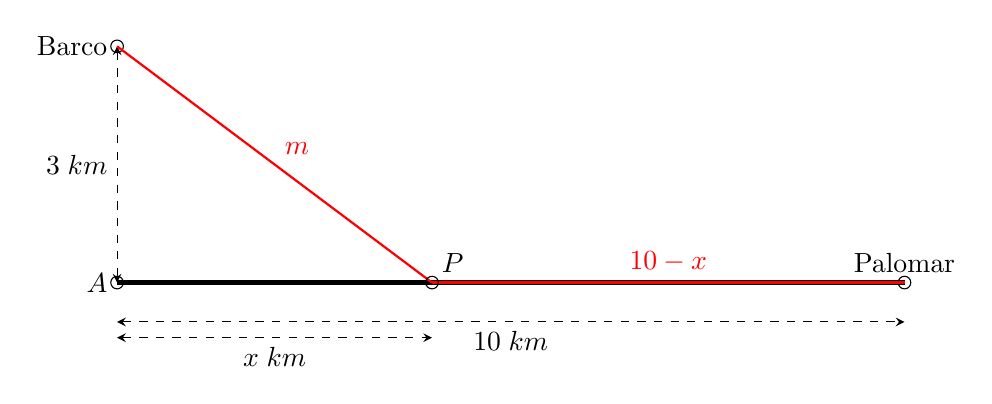
\begin{tikzpicture}
            \draw[ultra thick] (0,0) -- (10,0); % Costa
            
            \draw (0, 3) node[left] {Barco} circle (0.08);
            \draw[stealth-stealth, dashed] (0,3) -- node[left] {$3\; km$} (0,0);
            
            \draw (0, 0) node[left] {$A$} circle (0.08);

            \draw (10, 0) node[above] {Palomar} circle (0.08);
            \draw[stealth-stealth, dashed] (0,-0.5) -- node[below] {$10\; km$} (10,-0.5);

            \def\p{4}
            \draw[thick, red] (0,3) -- node[above right] {$m$} (\p,0);
            \draw[thick, red] (\p,0) -- node[above] {$10-x$} (10,0);

            \draw (\p, 0) node[above right] {$P$} circle (0.08);
            \draw[stealth-stealth, dashed] (0,-0.7) -- node[below] {$x\; km$} (\p,-0.7);
        \end{tikzpicture}
    \end{figure}

    La ecuación de ligadura, por el Teorema de Pitágoras, es:
    \begin{equation*}
        m^2 = 3^2 + x^2 \Longrightarrow m=\sqrt{9+x^2}
    \end{equation*}

    La función que determina la energía consumida es:
    \begin{equation*}
        \begin{array}{rl}
            E:]0, 10[ & \longrightarrow \bb{R}\\
                    x & \longrightarrow E(x) = 2m + (10-x) = 2\sqrt{9+x^2} + 10-x
        \end{array}
    \end{equation*}

    \begin{equation*}
        E'(x) = 2\frac{2x}{2\sqrt{9+x^2}} - 1 = \frac{2x}{\sqrt{9+x^2}} - 1
    \end{equation*}
    \begin{equation*}
        E'(x)= 0 \Longleftrightarrow 2x=\sqrt{9+x^2} \Longleftrightarrow 4x^2 = 9+x^2 \Longleftrightarrow x=\sqrt{3}\;km
    \end{equation*}
    Veamos si, efectivamente, el punto crítico es extremo relativo.
    \begin{itemize}
        \item \underline{Para $x<\sqrt{3}$}: $E'(x) < 0 \Longrightarrow E(x)$ estrictamente decreciente.
        \item \underline{Para $x>\sqrt{3}$}: $E'(x) > 0 \Longrightarrow E(x)$ estrictamente creciente.
    \end{itemize}

    Por tanto, sí es extremo relativo. Además, es absoluto ya que es el único extremo relativo y la función es continua y el dominio es un intervalo.
    
    Por tanto, el punto pedido $P$ se encuentra a $\sqrt{3}\;km$ del punto $A$ en la costa.
\end{ejercicio}

\begin{ejercicio}
    Se inscribe un rectángulo en la elipse $\frac{x^2}{400} + \frac{y^2}{225} = 1$ con sus lados paralelos a los ejes. Hállense las dimensiones del rectángulo para que:
    \begin{enumerate}
        \item El área sea máxima.
        \begin{figure}[H]
            \centering
            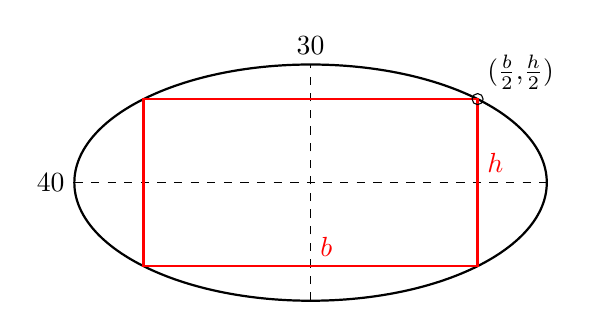
\begin{tikzpicture}
                % define los ejes de la elipse
                \def\a{3}
                \def\b{1.5}
                
                % dibuja la elipse
                \draw[thick] (0,0) ellipse (\a cm and \b cm);
                \draw[dashed] (0,-\b) -- (0,\b);
                \draw[dashed] (-\a,0) -- (\a, 0);
                \node at (0, \b)[above] {$30$} ;
                \node at (-\a,0)[left] {$40$} ;
                
                % calcula las coordenadas de los vertices del rectangulo inscrito
                \pgfmathsetmacro{\x}{\a/sqrt(2)}
                \pgfmathsetmacro{\y}{\b/sqrt(2)}
                
                % dibuja el rectangulo inscrito
                \draw[thick,red] (-\x,-\y) rectangle (\x,\y);
                \node at (0, -\y)[above right, red] {$b$} ;
                \node at (\x, 0)[above right, red] {$h$} ;

                \draw (\x,\y) circle[radius=2pt]; % Dibuja un círculo en el punto (\x.\y)
                \draw (\x,\y) node[above right] {($\frac{b}{2}$,$\frac{h}{2}$)}; % Dibuja la etiqueta con las coordenadas
            \end{tikzpicture}
        \end{figure}
        Dada la ecuación de la elipse, sabemos que el semieje mayor mide $\sqrt{400}=20$, y el semieje menor mide $\sqrt{225}=15$.

        La ecuación de ligadura es que el punto $\left(\frac{b}{2}, \frac{h}{2}\right)$ pertenece a la elipse, por lo que cumple la ecuación. Es decir, la ecuación de ligadura es:
        \begin{equation*}
            \frac{\left(\frac{b}{2}\right)^2}{400} + \frac{\left(\frac{h}{2}\right)^2}{225} = 1 \Longrightarrow b = \sqrt{1600 \left(1 - \frac{h^2}{900} \right)} \Longrightarrow b= 40 \sqrt{1 - \frac{h^2}{900}}
        \end{equation*}
        La función a maximizar es el área del rectángulo, es decir,
        \begin{equation}\label{Ej4.1}
            \begin{array}{rl}
                A:]0, 30[ & \longrightarrow \bb{R}\\
                        h & \longrightarrow A(h) = b\cdot h = 40h \sqrt{1 - \frac{h^2}{900}}
            \end{array}
        \end{equation}

        Para maximizar $A$, es decir, calcular su máximo, calculamos los extremos relativos.
        $$A'(h) = 40\sqrt{1 - \frac{h^2}{900}} + 40h\frac{\frac{-h}{450}}{2\sqrt{1 - \frac{h^2}{900}}}
        = 40\sqrt{1 - \frac{h^2}{900}} - \frac{2h^2}{45\sqrt{1 - \frac{h^2}{900}}}
        $$
        \begin{multline*}
            A'(x) = 0\Longrightarrow
            900\sqrt{1 - \frac{h^2}{900}} = \frac{h^2}{\sqrt{1 - \frac{h^2}{900}}}
            \Longrightarrow 900^2 -900h^2 = \frac{h^4}{1-\frac{h^2}{900}} \Longrightarrow\\
            \Longrightarrow 900^2 - 900h^2 -900h^2 +\cancel{h^4} = \cancel{h^4} \Longrightarrow\\\Longrightarrow 900(-2h^2 + 900)=0 \Longrightarrow h= 15\sqrt{2}
        \end{multline*}
        Veamos ahora si el punto crítico $h=15\sqrt{2}$ es efectivamente un máximo relativo.
        \begin{itemize}
            \item \underline{Para $h<15\sqrt{2}$} $A'(h) > 0 \Longrightarrow A$ estrictamente creciente.
            \item \underline{Para $h>15\sqrt{2}$} $A'(h) < 0 \Longrightarrow A$ estrictamente decreciente.
        \end{itemize}
        Por tanto, efectivamente obtenemos un máximo relativo en $h=15\sqrt{2}\;u.$ El valor de la base es $b=20\sqrt{2}\;u.$ El área para estas dimensiones es $A=600\;u^2$.

        Además, efectivamente obtenemos un máximo absoluto, ya que
        $$\lim_{h\to 0^+}A(h) = \lim_{h\to 30^-}A(h) = 0 < A(15\sqrt{2}) = 600\;u^2$$

        Por tanto, las dimensiones pedidas son:
        $$b=20\sqrt{2}\;u \qquad h=15\sqrt{2}\;u \qquad A=600\;u^2$$
        
        \item El perímetro sea máximo.\\
        En este caso, la función a maximizar es el perímetro del rectángulo, es decir,
        \begin{equation}\label{Ej4.2}
            \begin{array}{rl}
                P:]0, 30[ & \longrightarrow \bb{R}\\
                        h & \longmapsto P(h) = 2b + 2h = 80\sqrt{1 - \frac{h^2}{900}} + 2h
            \end{array}
        \end{equation}

        Para maximizar $P$, es decir, calcular su máximo, calculamos los extremos relativos.
        $$P'(h) = 80\frac{\frac{-h}{450}}{2\sqrt{1 - \frac{h^2}{900}}} +2
        = -\frac{4h}{45\sqrt{1 - \frac{h^2}{900}}} +2
        $$
        \begin{multline*}
            P'(x) = 0\Longrightarrow
            2=\frac{4h}{45\sqrt{1 - \frac{h^2}{900}}} \Longrightarrow 90\sqrt{1 - \frac{h^2}{900}} = 4h
            \Longrightarrow\\ \Longrightarrow
            90^2 \left(1 - \frac{h^2}{900}\right) = 16h^2
            \Longrightarrow 90^2 - 9h^2 = 16h^2 \Longrightarrow h=18 \; u.
        \end{multline*}
        Veamos ahora si el punto crítico $h=18$ es efectivamente un máximo relativo.
        \begin{itemize}
            \item \underline{Para $h<18$} $P'(h) > 0 \Longrightarrow P$ estrictamente creciente.
            \item \underline{Para $h>18$} $P'(h) < 0 \Longrightarrow P$ estrictamente decreciente.
        \end{itemize}
        Por tanto, efectivamente obtenemos un máximo relativo en $h=18\;u.$ El valor de la base es $b=32\;u.$ El perímetro para estas dimensiones es $P(18)=~100\;u$.

        Además, efectivamente obtenemos un máximo absoluto, ya que
        $$\lim_{h\to 0^+}P(h) = \lim_{h\to 30^-}P(h) = 0 < P(18) =100\;u$$

        Por tanto, las dimensiones pedidas son:
        $$b=32\;u \qquad h=18\;u \qquad P=100\;u$$
    \end{enumerate}
\end{ejercicio}

\begin{ejercicio}
    Se desea confeccionar una tienda de campaña cónica de un volumen determinado. Calcúlense sus dimensiones para que la cantidad de lona necesaria sea mínima.
    \begin{figure}[H]
        \centering
        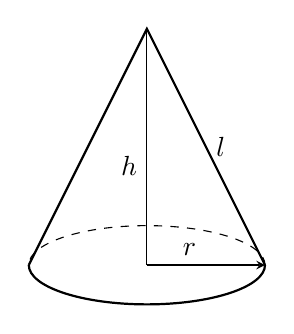
\begin{tikzpicture}
            \def\r{1.5}
            \def\b{0.5}
            \def\h{3}
        
            % dibuja la elipse
            \draw[thick] (-\r, 0) -- (0,\h) -- node[right] {$l$} (\r, 0) ;
            \draw[thick] (-\r,0) arc (180:360:\r cm and \b cm);
            \draw[dashed] (\r,0) arc (0:180:\r cm and \b cm);

            \draw (0,0) -- node[below left] {$h$} (0,\h);
            \draw[-stealth] (0,0) -- node[above left] {$r$} (\r,0);
        \end{tikzpicture}
    \end{figure}

    Cabe destacar que se toma como lona solo la superficie lateral. La superficie para la base no se tiene en cuenta.
    
    En este caso, tengo varias ecuaciones de ligadura. En primer lugar,
    $$V_o = cte = \frac{1}{3}\pi r^2h \Longrightarrow h = \frac{3V_0}{\pi r^2}$$

    En segundo lugar, por el Teorema de Pitágonas,
    $$l^2 = r^2 + h^2 \Longrightarrow l = \sqrt{r^2 + h^2} = \sqrt{r^2 + \frac{9V_0^2}{\pi^2r^4}}$$

    Por tanto, la función a minimizar es:
    \begin{equation*}
        \begin{array}{rl}
            A:\bb{R^+} & \longrightarrow \bb{R}\\
                    r & \longmapsto A(r)
        \end{array}
    \end{equation*}
    \begin{equation*}
        A(r) = \pi rl = \pi r\sqrt{r^2 + \frac{9V_0^2}{\pi^2r^4}}
    \end{equation*}

    Como $A(r)>0\;\forall r$, calculo los puntos críticos de $A^2(r)$, ya que alcanzan los extremos relativos en los mismos puntos.
    \begin{equation*}
        A^2(r) = \pi^2 r^2 \left( r^2 + \frac{9V_0^2}{\pi^2r^4}\right) = \pi^2 r^4 + \frac{9V_0^2}{r^2}
    \end{equation*}
    \begin{equation*}
        (A^2)'(r) = 4\pi^2r^3 - \frac{18V_0^2}{r^3} \Longrightarrow (A^2)'(r) = 0\Longleftrightarrow 4\pi^2r^6 = 18V_0^2 \Longleftrightarrow r=\sqrt[6]{\frac{9V_0^2}{2\pi^2}}
    \end{equation*}

    Una vez obtenido el punto crítico, comprobamos si es un mínimo relativo.
    \begin{equation*}
        (A^2)''(r) = 12\pi^2r^2 + \frac{54V_0^2}{r^4} >0 \qquad \forall r\in \bb{R}^+
    \end{equation*}

    Por tanto, como la segunda derivada es positiva, se trata de un mínimo relativo. También es absoluto, ya que la función es continua definida en un intervalo y es el único extremo relativo. Por tanto, como es mínimo absoluto de $A^2$, también lo es de $A$.
    
    Las dimensiones pedidas son, por tanto,
    \begin{equation*}
         r=\sqrt[6]{\frac{9V_0^2}{2\pi^2}} \qquad h=\frac{3V_0}{\pi \sqrt[6]{\left(\frac{9V_0^2}{2\pi^2}\right)^2}}
    \end{equation*}
\end{ejercicio}

\begin{ejercicio}
    Demuéstrese que la suma de un número positivo y su inverso es mayor o igual a 2.\\

    Sea $x\in \bb{R}^+$ el número referido. Se pide demostrar que $x+\frac{1}{x} \geq 2 \quad \forall x\in \bb{R}^+$. Sea $f$ la función:
    \begin{equation*}
        \begin{array}{rl}
            f:\bb{R^+} & \longrightarrow \bb{R}\\
                    x & \longmapsto f(x)=x+\frac{1}{x}
        \end{array}
    \end{equation*}
    \begin{equation*}
        f'(x)=1-\frac{1}{x^2} = 0\Longleftrightarrow x^2=1 \Longleftrightarrow x=1
    \end{equation*}

    \begin{itemize}
        \item \underline{Para $x<1$:}\\
        $f'(x)<0 \Longrightarrow f$ estrictamente decreciente.
        \item \underline{Para $x>1$:}\\
        $f'(x)>0 \Longrightarrow f$ estrictamente creciente.
    \end{itemize}

    Por tanto, $x=1$ es un mínimo relativo. Además, es también un mínimo absoluto, ya que es el único extremo relativo y
    $$\lim_{x\to0^+}f(x)= \lim_{x\to+\infty}f(x) = +\infty$$

    Por tanto, el número positivo cuya suma es la menor es $x=1$. Dicha suma mínima es $f(1)=2$, como se pedía demostrar.
\end{ejercicio}

\begin{ejercicio}
    Hállense las dimensiones del cilindro de mayor volumen entre todos aquellos que tienen la superficie total constante.
    \begin{figure}[H]
        \centering
        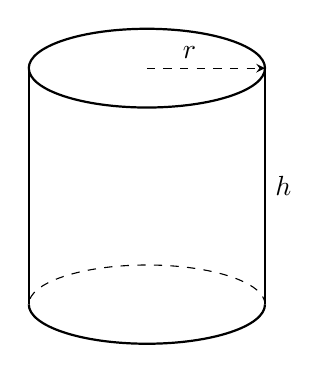
\begin{tikzpicture}
            \def\r{1.5}
            \def\b{0.5}
            \def\h{3}
        
            \draw[thick] (-\r, 0) -- (-\r,\h);
            \draw[thick] (\r, 0) -- node[right] {$h$} (\r,\h);
            
            \draw[thick] (-\r,0) arc (180:360:\r cm and \b cm);
            \draw[dashed] (\r,0) arc (0:180:\r cm and \b cm);

            \draw[thick] (-\r,\h) arc (180:360:\r cm and \b cm);
            \draw[thick] (\r,\h) arc (0:180:\r cm and \b cm);

            \draw[-stealth, dashed] (0,\h) -- node[above left] {$r$} (\r,\h);
        \end{tikzpicture}
    \end{figure}

    La ecuación de ligadura es:
    \begin{equation*}
        S_{T} = S_{Lat} + 2\cdot S_{Tapa} = 2\pi r h +2\pi r^2 = 2\pi r(h+r)\Longrightarrow h=\frac{S_T}{2\pi r} -r
    \end{equation*}

    El volumen a maximizar es:
    \begin{equation*}
        \begin{array}{rl}
            V:\bb{R^+} & \longrightarrow \bb{R}\\
                    r & \longmapsto V(r)=\pi r^2h = \pi r^2 \left(\frac{S_T}{2\pi r} -r\right)
                    = \frac{S_T}{2}r -\pi r^3
        \end{array}
    \end{equation*}
    \begin{equation*}
        V'(r)=\frac{S_T}{2}-3\pi r^2 = 0 \Longleftrightarrow r=\sqrt{\frac{S_T}{6\pi}}
    \end{equation*}

    Como $V''(r)=-6\pi r<0\quad \forall r$, tengo que $r=\sqrt{\frac{S_T}{6\pi}}$ es un máximo relativo. Además, es absoluto por ser el único extremo relativo de una función continua, derivable y definida en un intervalo.

    Por tanto, las dimensiones son:
    \begin{equation*}
        r=\sqrt{\frac{S_T}{6\pi}}
    \end{equation*}
    \begin{multline*}
        h=\frac{S_T}{2\pi r} -r
        =\frac{S_T}{2\pi \sqrt{\frac{S_T}{6\pi}}} -\sqrt{\frac{S_T}{6\pi}}
        =\sqrt{\frac{S_T^2}{\frac{4S_T\pi^2}{6\pi}}} -\sqrt{\frac{S_T}{6\pi}}
        =\\=
        \sqrt{\frac{3S_T}{2\pi}} -\sqrt{\frac{S_T}{6\pi}} = \sqrt{\frac{S_T}{\pi}}\left(\sqrt{\frac{3}{2}} - \sqrt{\frac{1}{6}}\right)
        = \sqrt{\frac{S_T}{\pi}}\cdot \frac{\sqrt{6}}{3} = \sqrt{\frac{2S_T}{3\pi}}
    \end{multline*}
\end{ejercicio}

\begin{ejercicio}
    Se desea construir un silo, con un volumen $V$ determinado, que tenga la forma de un cilindro rematado por una semiesfera. El costo de construcción (por unidad de superficie) es doble para la semiesfera que para el cilindro (la base es gratis). Determínense las dimensiones óptimas para minimizar el costo de construcción.
    \begin{figure}[H]
        \centering
        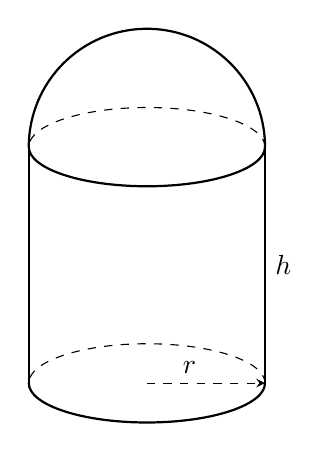
\begin{tikzpicture}
            \def\r{1.5}
            \def\b{0.5}
            \def\h{3}
        
            \draw[thick] (-\r, 0) -- (-\r,\h);
            \draw[thick] (\r, 0) -- node[right] {$h$} (\r,\h);
            
            \draw[thick] (-\r,0) arc (180:360:\r cm and \b cm);
            \draw[dashed] (\r,0) arc (0:180:\r cm and \b cm);

            \draw[thick] (-\r,\h) arc (180:360:\r cm and \b cm);
            \draw[dashed] (\r,\h) arc (0:180:\r cm and \b cm);

            \draw[thick] (\r,\h) arc (0:180:\r cm and \r cm);

            \draw[dashed, -stealth] (0,0) -- node[above left] {$r$} (\r,0);
        \end{tikzpicture}
    \end{figure}
    En este caso, la ecuación de ligadura es el volumen.
    \begin{equation*}
        V = V_{cilindro} + V_{esfera} = \pi r^2h + \frac{4}{6}\pi r^3 \Longrightarrow h=\frac{V-\frac{2}{3}\pi r^3}{\pi r^2}
    \end{equation*}
    Sea $C$ la función que representa los costes de producción a minimizar:
    \begin{equation*}
        \begin{array}{rl}
            C:\bb{R^+} & \longrightarrow \bb{R}\\
                    r & \longmapsto C(r)
        \end{array}
    \end{equation*}
    \begin{equation*}\begin{split}
        C(r)&=S_{Lat} + 2\cdot S_{esfera} = 2\pi rh + 4\pi r^2 = 2\pi r\frac{V-\frac{2}{3}\pi r^3}{\pi r^2} + 4\pi r^2\\
        &= \frac{2V}{r} - \frac{4}{3}\pi r^2 + 4\pi r^2 = \frac{2V}{r} + \frac{8}{3}\pi r^2
    \end{split}\end{equation*}
    \begin{equation*}
        C'(r) = -\frac{2V}{r^2} + \frac{16}{3}\pi r = 0 \Longleftrightarrow 3V = 8\pi r^3 \Longleftrightarrow r=\sqrt[3]{\frac{3V}{8\pi}} \text{ punto crítico}.
    \end{equation*}

    Veamos ahora si el punto crítico es extremo relativo.
    \begin{equation*}
        C''(r) = \frac{4V}{r^3} +\frac{16}{3}\pi > 0 \qquad \forall r\in \bb{R}^+.
    \end{equation*}
    Por tanto, efectivamente el valor de $r$ es un mínimo relativo. Además, es absoluto por ser el único extremo relativo y ser la función definida en un intervalo y continua en este.

    Por tanto, las dimensiones óptimas son:
    \begin{equation*}
        r=\sqrt[3]{\frac{3V}{8\pi}} \qquad h=\frac{V-\frac{1}{4}V}{\pi r^2} = \frac{V}{4\pi r^2}
    \end{equation*}
\end{ejercicio}

\begin{ejercicio}
    Se proyecta un jardín de forma de sector circular de radio $r$ y ángulo central $q$. El área del jardín, $A$, ha de ser fija. ¿Qué valores de $r$ y $q$ hacen mínimo el perímetro que bordea el jardín?
    \begin{figure}[H]
        \centering
        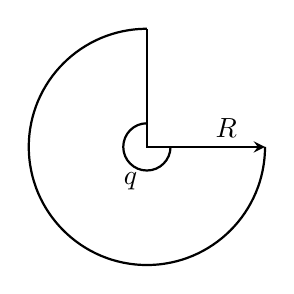
\begin{tikzpicture}
            \def\r{1.5}
            \def\q{0.3}

            \draw[thick] (0,0) arc (90:360:\r);
            \draw[thick] (0,-\r+\q) arc (90:360:\q);
            \draw[-stealth, thick] (0,0) -- (0, -\r) -- (\r, -\r);
            
            \draw (\r/2, -\r) node[above right] {$R$};
            \draw (0, -\r-0.2) node[below left] {$q$};            
        \end{tikzpicture}
    \end{figure}

    La ecuación de ligadura, en este caso, es que el área es fija.
    \begin{equation*}
        A = \frac{q}{2\pi} \pi r^2\Longrightarrow q=\frac{2A}{r^2}
    \end{equation*}

    Por tanto, la función que representa el perímetro es:
    \begin{equation*}
        \begin{array}{rl}
            P:\bb{R^+} & \longrightarrow \bb{R}\\
                    r & \longmapsto P(r)= 2r + \frac{q}{2\pi}2\pi r = 2r + \frac{2A}{r}
        \end{array}
    \end{equation*}
    \begin{equation*}
        P'(r)=2 -\frac{2A}{r^2} = 0 \Longleftrightarrow r^2=A \Longleftrightarrow r=\sqrt{A}
    \end{equation*}
    \begin{itemize}
        \item \underline{Para $r<\sqrt{A}$} $P'(r)<0 \Longrightarrow P(r)$ estrictamente decreciente.
        \item \underline{Para $r>\sqrt{A}$} $P'(r)>0 \Longrightarrow P(r)$ estrictamente creciente.
    \end{itemize}
    Por tanto, como se produce un cambio en el crecimiento, $r=\sqrt{A}$ es un mínimo relativo. Además, es absoluto, ya que la función es continua, el dominio es un intervalo, y es el único extremo relativo que hay.
    
    Por tanto, las dimensiones pedidas son:
    \begin{equation*}
        q=2\;\text{radianes} \qquad r=\sqrt{A}
    \end{equation*}
\end{ejercicio}

\begin{ejercicio}
    Una persona desea cortar un pedazo de alambre de 1 metro de largo en dos trozos. Uno de ellos se va a doblar en forma de circunferencia, y el otro en forma de cuadrado ¿Cómo debe cortar el alambre para que la suma de áreas sea mínima?
    \begin{figure}[H]
        \centering
        \begin{tikzpicture}
            \def\r{1.3};
            \def\l{2.6};

            \draw (0,\r) circle (\r);
            \draw (\r+1,0) rectangle (\r+1+\l, \l);

            \draw[-stealth, dashed] (0,\r) -- node[above] {$r$} (\r,\r);
            \node at(\r+1+\l, \l/2) [right] {$l$};
        \end{tikzpicture}
    \end{figure}

    En este caso, la ecuación de ligadura es la longitud del alambre.
    \begin{equation*}
        P=1\;m = P_{\bigcirc} + P_{\Box} = 2\pi r + 4l \Longrightarrow l=\frac{1-2\pi r}{4} = \frac{1}{4} - \frac{1}{2}\pi r
    \end{equation*}

    La función que representa el área total a minimizar es:
    \begin{equation*}
        \begin{array}{rl}
            A_T:]0,1[ & \longrightarrow \bb{R}\\
                    l & \longmapsto A_T(l)= A_{\bigcirc} + A_{\Box} = \pi r^2 + l^2 = \pi r^2 + \frac{1}{8} + \frac{\pi ^2 r^2}{4} - \frac{1}{4}\pi r
        \end{array}
    \end{equation*}
    \begin{equation*}
        A_T' = 2\pi r + \frac{\pi ^2 r}{2} - \frac{\pi}{4} = 0 \Longleftrightarrow r=\frac{\frac{\pi}{4}}{2\pi + \frac{\pi^2}{2}} = \frac{1}{8 + 2\pi}\; m
    \end{equation*}

    Comprobemos si el punto crítico efectivamente es extremo relativo.
    \begin{equation*}
        A_T''(r) = 2\pi + \frac{\pi^2}{2} > 0\qquad  \forall r \in ]0,1[
    \end{equation*}

    Por tanto, es un mínimo relativo. Además, es absoluto, ya que es el único extremo relativo y la función es continua definida en un intervalo.

    Por tanto, las medidas pedidas son:
    \begin{equation*}
        r=\frac{1}{8+2\pi}\;m \qquad l=\frac{1}{4} - \frac{\pi}{16+4\pi}\;m
    \end{equation*}

    Por tanto, los trozos de alambre serán de:
    \begin{equation*}
        P_{\bigcirc} = 2\pi r = \frac{2\pi}{8+2\pi} = \frac{\pi}{4+\pi}\;m
        \qquad
        P_{\Box} = 4l = 4\cdot \left(\frac{1}{4} - \frac{\pi}{16+4\pi}\right) = 1-\frac{\pi}{4+\pi} = \frac{4}{4+\pi}\;m
    \end{equation*}
\end{ejercicio}

\begin{ejercicio}
    Un muro de 4 metros de altura está a 3 metros de la fachada de una casa. Hallar la escalera más corta que llegará desde el suelo hasta la casa por encima del muro.
    \begin{figure}[H]
        \centering
        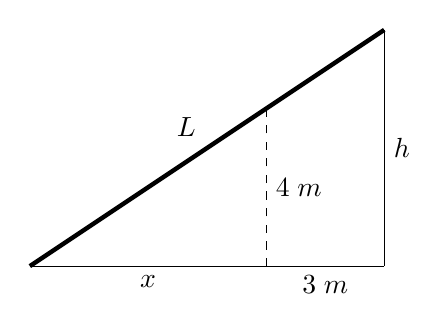
\begin{tikzpicture}
            \def\h{3};
            \def\x{3};
            \def\m{2};
            \def\d{1.5};
            

            \draw (0,0) -- node[below] {$x$} (\x,0) -- node[below] {$3\;m$} (\x+\d,0) ;
            \draw (\x+\d,0) -- node[right] {$h$} (\x+\d,\h);
            \draw [ultra thick] (\x+\d,\h) -- node[above left] {$L$} (0,0);
            \draw [dashed] (\x,0) -- node[right]{$4\;m$} (\x, \m);
        \end{tikzpicture}
    \end{figure}
    En este caso, la ecuación de ligadura viene dada por el Teorema de Thales:
    \begin{equation*}
        \frac{h}{4} = \frac{3+x}{x} \Longrightarrow h=4\cdot \frac{3+x}{x}
    \end{equation*}

    La función $L$ que determina la longitud de la escalera viene dada por:
    \begin{equation*}
        \begin{array}{rl}
            L:\bb{R^+} & \longrightarrow \bb{R}\\
                    x & \longmapsto L(x)= \sqrt{h^2 + (3+x)^2} = \sqrt{\left(4\cdot \frac{3+x}{x}\right)^2 + (3+x)^2}
        \end{array}
    \end{equation*}
    Como $L(x)\geq 0 \;\forall x \in \bb{R}^+ $, minimizo $L^2(x)$, ya que tendrá el mismo mínimo absoluto.
    \begin{equation*}
        (L^2)'(x) = 32\cdot \frac{3+x}{x}\cdot \frac{x-3-x}{x^2} + 2(3+x) = -96\cdot \frac{3+x}{x^3} + 6 + 2x
    \end{equation*}
    \begin{multline*}
        (L^2)'(x) = 0\Longleftrightarrow 96(3+x) = 6x^3 + 2x^4 \Longleftrightarrow x^4 + 3x^3 -48x -144=0
        \Longleftrightarrow \\ \stackrel{Fig.\;\ref{Fig:Ej11:DivRuffini}}{\Longleftrightarrow}
        (x+3)(x^3-48) = 0 \Longleftrightarrow x=\{\cancel{-3}, \sqrt[3]{48}\}
    \end{multline*}

    \begin{figure}[H]
        \centering
        \polyhornerscheme[x=-3]{x^4+3x^3-48x-144}
        \caption{División mediante Ruffini donde se ve que $x=-3$ es una solución.}
        \label{Fig:Ej11:DivRuffini}
    \end{figure}

    Como $L^2(x)$ es derivable en $\bb{R}^+$, comprobemos que $x= \sqrt[3]{48}$ es extremo relativo:
    \begin{itemize}
        \item \underline{Para $0<x<\sqrt[3]{48}$} $(L^2)'(x)<0 \Longrightarrow L^2(x)$ decrece.
        \item \underline{Para $\sqrt[3]{48}<x$} $(L^2)'(x)>0 \Longrightarrow L^2(x)$ crece.
    \end{itemize}

    Por tanto, efectivamente es un mínimo relativo. Además, es absoluto, ya que es el único extremo relativo de una función continua y derivable en un intervalo.

    Por tanto, la longitud de la escalera es:
    \begin{multline*}
        L(\sqrt[3]{48}) = \sqrt{\left(4\cdot \frac{3+\sqrt[3]{48}}{\sqrt[3]{48}}\right)^2 + (3+\sqrt[3]{48})^2}
        = \sqrt{\left(4\cdot \frac{3+\sqrt[3]{48}}{\sqrt[3]{48}}\right)^2\left(1+\frac{\sqrt[3]{48}}{4}\right)}
        =\\= 4\cdot \frac{3+\sqrt[3]{48}}{\sqrt[3]{48}}\sqrt{1+\frac{\sqrt[3]{48}}{4}} \approx 10.0877\;m
    \end{multline*}        
\end{ejercicio}

\begin{ejercicio}
    Demuéstrese que de todos los triángulos isósceles que se pueden circunscribir a una circunferencia de radio $r$ el de área mínima es el triángulo equilátero de altura $3r$.
    \begin{figure}[H]
        \centering
        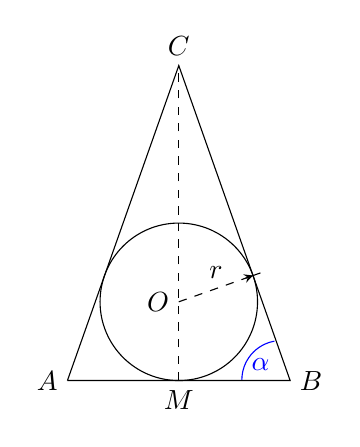
\begin{tikzpicture}
            
            \def\r{1};
            \pgfmathsetmacro{\x}{\r*sqrt(2)};
            \pgfmathsetmacro{\h}{3*\r};

            \pgfmathsetmacro{\ang}{19.48};
            
            \pgfmathsetmacro{\px}{\r*cos(\ang)};
            \pgfmathsetmacro{\py}{\r*sin(\ang)};

            \draw (0,0) circle (\r);
            \draw (-\x, -\r) -- (\x, -\r) -- (0, \h) -- (-\x, -\r);

            \draw[-stealth, dashed] (0,0) -- node[above]{$r$} (\px, \py);
            \draw (0.9*\px, 0.9*\py) -- (1.1*\px, 1.1*\py);
            \draw[dashed] (0, -\r) -- (0, \h);

            \node [above] at (0, \h) {$C$};
            \node [right] at (\x, -\r) {$B$};
            \node [left] at (-\x, -\r) {$A$};
            \node [below] at (0, -\r) {$M$};
            \node [left] at (0,0) {$O$};

            \draw[blue] (\x-0.2,-\r+0.5) arc (100:180:0.5) node[above right] {$\alpha$};
        \end{tikzpicture}
    \end{figure}

    Como es isósceles, tenemos que $\alpha = \angle CAB = \angle CBA$. Además, tenemos que $\overline{AC}=\overline{CB}$. Además, $\overline{AB}=2\overline{AM}=2\overline{BM}$.

    Nos reducimos a $\triangle OBM$.
    \begin{figure}[H]
        \centering
        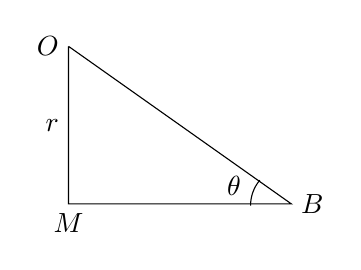
\begin{tikzpicture}
            
            \def\r{2};
            \pgfmathsetmacro{\x}{\r*sqrt(2)};
            \pgfmathsetmacro{\h}{3*\r};

            \pgfmathsetmacro{\ang}{19.48};
            
            \pgfmathsetmacro{\px}{\r*cos(\ang)};
            \pgfmathsetmacro{\py}{\r*sin(\ang)};

            
            \draw (0,0) -- (\x,-\r) -- (0,-\r) -- node[left] {$r$}(0,0);

            
            \node [right] at (\x, -\r) {$B$};
            \node [below] at (0, -\r) {$M$};
            \node [left] at (0,0) {$O$};

            \draw (\x-0.4,-\r+0.3) arc (140:180:0.5) node[above left] {$\theta$};
        \end{tikzpicture}
    \end{figure}
    Una de las ecuaciones de ligadura es:
    \begin{equation*}
        \tan \theta = \tan \frac{\alpha}{2} = \frac{r}{\overline{BM}} \Longrightarrow \overline{BM} = \frac{r}{\tan \frac{\alpha}{2}}
    \end{equation*}

    Nos reducimos ahora a $\triangle CBM$.
    \begin{figure}[H]
        \centering
        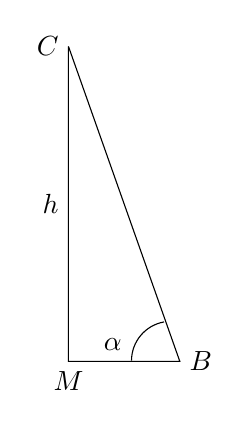
\begin{tikzpicture}
            
            \def\r{1};
            \pgfmathsetmacro{\x}{\r*sqrt(2)};
            \pgfmathsetmacro{\h}{3*\r};

            \pgfmathsetmacro{\ang}{19.48};
            
            \pgfmathsetmacro{\px}{\r*cos(\ang)};
            \pgfmathsetmacro{\py}{\r*sin(\ang)};

            
            \draw (0,\h) -- (\x,-\r) -- (0,-\r) -- node[left] {$h$}(0,\h);

            
            \node [right] at (\x, -\r) {$B$};
            \node [below] at (0, -\r) {$M$};
            \node [left] at (0,\h) {$C$};

            \draw (\x-0.2,-\r+0.5) arc (100:180:0.5) node[above left] {$\alpha$};
        \end{tikzpicture}
    \end{figure}
    La otra de las ecuaciones de ligadura es:
    \begin{equation*}
        \tan \alpha = \frac{\overline{CM}}{\overline{BM}} \Longrightarrow \overline{CM} = h =  \tan \alpha \cdot \overline{BM} = \tan \alpha  \cdot \frac{r}{\tan \frac{\alpha}{2}} = r \cdot \frac{\tan \alpha}{\tan \frac{\alpha}{2}}
    \end{equation*}
    
    La función del área del triángulo es:
    \begin{equation*}
        \begin{array}{rl}
            A:\displaystyle  \left]0,\frac{\pi}{2}\right[ & \longrightarrow \bb{R}\\
                    \alpha & \longmapsto A(\alpha)= \frac{1}{2}bh = \frac{2\cdot \overline{BM}\cdot \overline{CM}}{2} = \frac{r}{\tan \frac{\alpha}{2}} \cdot r \cdot \frac{\tan \alpha}{\tan \frac{\alpha}{2}} = r^2\frac{\tan \alpha}{\tan^2 \frac{\alpha}{2}}
        \end{array}
    \end{equation*}

    Para calcular el mínimo absoluto, calculamos los puntos críticos:
    \begin{equation*}\begin{split}
        A'(\alpha) &= r^2\cdot \frac{(1+\tan^2 \alpha)\tan\cancel{^2} \frac{\alpha}{2}-\cancel{2}\tan \alpha \cancel{\tan \frac{\alpha}{2}}(1+\tan^2 \frac{\alpha}{2})\cdot \cancel{\frac{1}{2}}}{\tan\cancelto{3}{^4} \frac{\alpha}{2}} \\
        &= r^2\cdot \frac{\tan \frac{\alpha}{2}(1+\tan^2\alpha)-\tan\alpha(1+ \tan^2 \frac{\alpha}{2})}{\tan^3 \frac{\alpha}{2}}\\
         &= r^2\cdot \frac{\frac{\tan \frac{\alpha}{2}}{\cos^2 \alpha} - \frac{\tan \alpha}{\cos^2 \frac{\alpha}{2}}}{\tan^3 \frac{\alpha}{2}} = 0 \Longleftrightarrow  \frac{\tan \frac{\alpha}{2}}{\cos^2 \alpha}=\frac{\tan \alpha}{\cos^2 \frac{\alpha}{2}}
    \end{split}\end{equation*}

    Resuelvo la ecuación $A'(\alpha)=0$, sabiendo que todas las funciones trigonométricas toman valores positivos por ser $\alpha$ del primer cuadrante. Además, ninguna se anula ni se va a $+\infty$, ya que el intervalo es abierto.
    \begin{multline*}
        A'(\alpha)=0 \Longleftrightarrow  \frac{\tan \frac{\alpha}{2}}{\cos^2 \alpha}=\frac{\tan \alpha}{\cos^2 \frac{\alpha}{2}}
        \Longleftrightarrow
        \tan \frac{\alpha}{2}\cos^2 \frac{\alpha}{2} = \tan \alpha \cos^2 \alpha
        \Longleftrightarrow \\ \Longleftrightarrow
        \sen \frac{\alpha}{2}\cos \frac{\alpha}{2} = \sen \alpha \cos \alpha
        \Longleftrightarrow
        2\sen \frac{\alpha}{2}\cos \frac{\alpha}{2} = 2\sen \alpha \cos \alpha
        \Longleftrightarrow \\ \Longleftrightarrow
        \cancel{\sen \alpha} = 2\cancel{\sen \alpha} \cos \alpha \Longleftrightarrow \cos{\alpha} = \frac{1}{2} \Longleftrightarrow \alpha=\frac{\pi}{3}
    \end{multline*}

    Veamos ahora si, efectivamente, se trata de un mínimo relativo.
    \begin{itemize}
        \item \underline{Para $\alpha<\frac{\pi}{3}$}: $A'(\alpha)<0 \Longrightarrow A(\alpha)$ estrictamente decreciente.
        \item \underline{Para $\alpha>\frac{\pi}{3}$}: $A'(\alpha)>0 \Longrightarrow A(\alpha)$ estrictamente creciente.
    \end{itemize}
    Por tanto, vemos que en $\alpha=\frac{\pi}{3}$ se produce un cambio de monotonía, por lo que efectivamente es un mínimo relativo. Además, también es absoluto, al ser el único extremo relativo en una función continua y derivable definida en un intervalo.

    Calculamos ahora la altura del triángulo de área mínima:
    \begin{equation*}
        h=\overline{CM} = r\cdot \frac{\tan \alpha}{\tan \frac{\alpha}{2}} =r\cdot \frac{\tan \frac{\pi}{3}}{\tan \frac{\pi}{6}} = 3r
    \end{equation*}
    Por tanto, queda demostrado el enunciado.    
\end{ejercicio}

\begin{ejercicio}
    ¿Cuál es la longitud de la barra más larga que puede hacerse pasar horizontalmente a través de la esquina, en ángulo recto, que forman dos corredores de anchuras respectivas $a$ y $b$?
    \begin{figure}[H]
        \centering
        \begin{tikzpicture}
            
            \def\a{1};
            \def\b{2};
            \def\x{10}
            \def\y{4}

            \draw (0,0) -- (\x,0) -- (\x, -\y);
            \draw (0,-\a) -- (\x-\b,-\a) -- (\x-\b, -\y);

            \draw[ultra thick, red] (\x-3, 0) -- (\x, -3);
            \draw[dashed, blue] (\x-\b, 0) -- node[right] {$a$} (\x-\b, -\a);
            \draw[dashed, blue] (\x, -\a) -- node[above right] {$b$} (\x-\b, -\a);

            \draw[red] (\x-3, 0) circle (0.08) node[above left]{$A$} ;
            \draw[red] (\x-\b, -\a) circle (0.08) node[below left]{$C$} ;
            \draw[red](\x, -3) circle (0.08) node[right]{$B$} ;

            \draw[blue] (\x-3+0.5, 0) arc (360:315:0.5) node[right] {$\alpha$};
            \draw[blue] (\x-\b+0.5, -\a) arc (360:315:0.5) node[right] {$\alpha$};

            \draw[dashed, red] (\x-4, 0) -- (\x, -2);
            

            \draw[stealth-stealth, dashed] (0,0) -- node[left] {$a$} (0, -\a);
            \draw[stealth-stealth, dashed] (\x-\b,-\y) -- node[below] {$b$} (\x, -\y);
        \end{tikzpicture}
    \end{figure}

    La barra pedida es el segmento que pasa por los puntos $A$, $B$ y $C$. Variando el valor de $\alpha$, obtenemos un haz de segmentos. Paradójicamente, necesitamos minizar la longitud de la barra que pasa por los puntos $A$, $B$ y $C$ ya que, al ser la longitud de la barra constante, si no se usa la barra más corta, en algún momento del giro chocará contra las paredes de los corredores.

    Por tanto, la longitud a minimizar de la barra pedida es:
    $$L=\overline{AC} + \overline{CB}$$
    
    La ecuación de ligadura en este caso viene dada por el ángulo $\alpha$, ya que al ser los dos corredores perpendiculares y la anchura de cada uno constante, el ángulo es el mismo. Por tanto, como $\alpha = \alpha$, las medidas de los segmentos son:
    \begin{equation*}
       \cos \alpha = \frac{b}{\overline{CB}} \Longrightarrow \overline{CB} = \frac{b}{\cos \alpha} \qquad
       \sen \alpha = \frac{a}{\overline{AC}} \Longrightarrow \overline{AC} = \frac{a}{\sen \alpha}
    \end{equation*}

    Por tanto, la longitud $L$ de la barra viene dada por:
    \begin{equation*}
        \begin{array}{rl}
            L:\displaystyle  \left]0, \frac{\pi}{2}\right[ & \longrightarrow \bb{R}\\
                    \alpha & \longmapsto L(x)= \displaystyle \frac{b}{\cos \alpha} + \frac{a}{\sen \alpha}
        \end{array}
    \end{equation*}

    \begin{multline*}
        L'(\alpha) = b\frac{\sen(\alpha)}{\cos^2\alpha} - a\frac{\cos\alpha}{\sen^2\alpha} = 0 \Longleftrightarrow b\frac{\sen(\alpha)}{\cos^2\alpha} = a\frac{\cos\alpha}{\sen^2\alpha} \Longleftrightarrow b\sen^3\alpha = a\cos^3\alpha\\
        \Longleftrightarrow \tg^3\alpha = \frac{a}{b} \Longleftrightarrow \tg\alpha = \sqrt[3]{\frac{a}{b}} \Longleftrightarrow \alpha = \arctg \sqrt[3]{\frac{a}{b}}
    \end{multline*}

    Veamos ahora si el punto crítico es un extremo relativo.
    \begin{multline*}
        L''(\alpha) = b\frac{\cos^3\alpha +2\cos\alpha \sen^2\alpha}{\cos^4\alpha} - a\frac{-\sen^3\alpha -2\sen\alpha \cos^2\alpha}{\sen^4\alpha}= \\
        = b\frac{\cos^2\alpha +2 \sen^2\alpha}{\cos^3\alpha} - a\frac{-\sen^2\alpha -2 \cos^2\alpha}{\sen^3\alpha}
        = b\frac{1+\sen^2\alpha}{\cos^3\alpha} - a\frac{-1- \cos^2\alpha}{\sen^3\alpha} =\\
        = b\frac{2-\cos^2\alpha}{\cos^3\alpha} + a\frac{2- \sen^2\alpha}{\sen^3\alpha}
    \end{multline*}

    Por tanto, podemos ver que $L''(\alpha) > 0 \qquad \forall \alpha \in \left]0, \frac{\pi}{2}\right[$, ya que en dicho intervalo tanto el seno como el coseno son positivos (por lo que los denominadores son positivos). Respecto a los numeradores, tanto el seno como el coseno en dicho intervalo están acotadas entre $]0, 1[$, por lo que su cubo también lo estará. Como $a,b\in \bb{R}^+$ y las fracciones son positivas, la segunda derivada en dicho intervalo siempre es positiva.

    Como $L''(\alpha) > 0 \qquad \forall \alpha \in \left]0, \frac{\pi}{2}\right[ \Longrightarrow \alpha = \sqrt[3]{\frac{a}{b}}$ es un mínimo relativo. También es absoluto, ya que la función es continua y definida en un intervalo.

    La longitud pedida es:
    \begin{equation*}
        L\left(\sqrt[3]{\frac{a}{b}}\right) = \frac{b}{\cos\left( \arctg \sqrt[3]{\frac{a}{b}}\right)} + \frac{a}{\sen \left( \arctg \sqrt[3]{\frac{a}{b}}\right)}
    \end{equation*}
\end{ejercicio}

\begin{ejercicio}
    Determinar las dimensiones del cilindro circular recto de volumen máximo que puede inscribirse en un cono circular recto de radio $R$ y altura $H$.
    \begin{figure}[H]
        \centering
        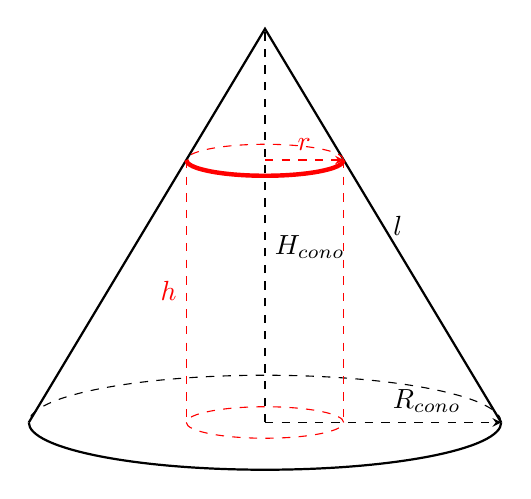
\begin{tikzpicture}
            \def\r{3}
            \def\b{0.6}
            \def\h{5}
            
            \def\radcirc{1/3*\r}
            \def\hcirc{2/3*\h}
            \def\a{0.2}
        
            % dibuja la elipse
            \draw[thick] (-\r, 0) -- (0,\h) -- node[right] {$l$} (\r, 0) ;
            \draw[thick] (-\r,0) arc (180:360:\r cm and \b cm);
            \draw[dashed] (\r,0) arc (0:180:\r cm and \b cm);

            \draw[dashed] (0,0) -- node[below right] {$H_{cono}$} (0,\h);
            \draw[-stealth, dashed] (0,0) -- node[above right] {$R_{cono}$} (\r,0);

            \draw[ultra thick, red] (-\radcirc,\hcirc) arc (180:360:\radcirc cm and \a cm);
            \draw[dashed, red] (\radcirc,\hcirc) arc (0:180:\radcirc cm and \a cm);

            \draw[dashed, red] (-\radcirc,0) arc (180:360:\radcirc cm and \a cm);
            \draw[dashed, red] (\radcirc,0) arc (0:180:\radcirc cm and \a cm);
            
            \draw[dashed, red] (-\radcirc,\hcirc) -- node[left]{$h$} (-\radcirc, 0);
            \draw[dashed, red] (\radcirc,\hcirc) -- (\radcirc, 0);
            \draw[dashed, red, -stealth] (0, \hcirc) -- node[above]{$r$} (\radcirc, \hcirc);
        \end{tikzpicture}
    \end{figure}
    La ecuación de ligadura viene dada por el Teorema de Thales:
    \begin{equation*}
        \frac{R_{cono}}{r} = \frac{H_{cono}}{H_{cono} - h} \Longrightarrow h=- \frac{H_{cono}r}{R_{cono}} + H_{cono}
    \end{equation*}

    La ecuación a maximizar es:
    \begin{equation*}
        \begin{array}{rl}
            V:]0, R_{cono}[ & \longrightarrow \bb{R}\\
                    r & \longmapsto V(r)= \pi r^2 h = \pi r^2\left(- \frac{H_{cono}r}{R_{cono}} + H_{cono}\right)
        \end{array}
    \end{equation*}
    \begin{equation*}
        V'(r) = 2\pi r\left(- \frac{H_{cono}r}{R_{cono}} + H_{cono}\right) -\frac{H_{cono}}{R_{cono}}\pi r^2 = -3\frac{H_{cono}}{R_{cono}}\pi r^2 + 2\pi r H_{cono}
    \end{equation*}
    \begin{equation*}
        V'(r)=0 \Longleftrightarrow \frac{3r}{R_{cono}} = 2 \Longleftrightarrow r=\frac{2}{3}R_{cono}
    \end{equation*}

    Veamos ahora si el punto crítico es, efectivamente, extremo relativo.
    \begin{equation*}
        V''(r) = -6\frac{H_{cono}}{R_{cono}}\pi r + 2\pi H_{cono} \qquad
        V''\left(\frac{2}{3}R_{cono}\right) = -4\pi H_{cono} + 2\pi H_{cono} < 0
    \end{equation*}

    Por tanto, como $V''(r) <0$ para el punto crítico, es un máximo relativo. Además, como la función es continua definida en un intervalo y solo tiene un extremo relativo, también es extremo absoluto.

    Por tanto, las dimensiones que maximizan el volumen del cilindro inscrito son:
    \begin{equation*}
        r=\frac{2}{3} R_{cono} \qquad h=-\frac{2}{3}H_{cono} + H_{cono} = \frac{1}{3}H_{cono}
    \end{equation*}
    
\end{ejercicio}

\begin{ejercicio}
    Un cultivador de naranjas estima que plantando 60 naranjos obtendría una cosecha media de 400 naranjas por árbol, y que este número bajaría 4 unidades por cada árbol más que se plante en el mismo terreno. Hállese el número de árboles que hace máxima la cosecha.\\

    Sea $P$ la función que determina la producción, es decir, el número de naranjas producidas. Sea $n$ el número de naranjos plantados, y $k$ el número de naranjas por árbol. La ecuación de ligadura es:
    $$k = 400 - 4(n-60) = 640 - 4n$$
    La función $P$ se define para $n\geq 60$, ya que en el caso de menos árboles no se da información sobre la productividad.
    \begin{equation*}
        \begin{array}{rl}
            P:[60, +\infty[ & \longrightarrow \bb{R}\\
                    n & \longmapsto P(n)=kn = 640n -4n^2
        \end{array}
    \end{equation*}
    \begin{equation*}
        P'(n) = 640 - 8n = 0\Longleftrightarrow n=80
    \end{equation*}

    Como $P''(n)=-8<0 \; \forall n\in [60, +\infty[$, efectivamente el punto crítico es un máximo relativo. Además, también es absoluto ya que la función es continua definida en un intervalo, y es el único extremo relativo que hay.

    Por tanto, el número de árboles que maximiza la cosecha son $n=80$ naranjos, siendo la cosecha total $P(80)=25600$ naranjas.
\end{ejercicio}

\begin{ejercicio}
    Durante la tos, el diámetro de la tráquea disminuye. La velocidad $v$ del aire en la tráquea durante la tos se relaciona con el radio $r$ mediante la ecuación $v=Ar^2(r_0-r)$, donde $A$ es una constante y $r_0$ es el radio en estado de relajación. Determínese el radio de la tráquea cuando la velocidad es máxima, así como esta velocidad.\\

    La función a maximizar es:
    \begin{equation*}
        \begin{array}{rl}
            V:]0, r_0[ & \longrightarrow \bb{R}\\
                    r & \longmapsto V(r)=Ar^2(r_0 - r) = Ar_0r^2 - Ar^3
        \end{array}
    \end{equation*}
    \begin{equation*}
        V'(r) = 2Ar_0r - 3Ar^2 = 0 \Longleftrightarrow r=\frac{2}{3}r_0
    \end{equation*}
    Veamos si el punto crítico es, efectivamente, un extremo relativo.
    \begin{equation*}
        V''(r) = 2Ar_0 - 6Ar \Longrightarrow V''\left(\frac{2}{3}r_0\right) = 2Ar_0 - 4Ar_0 = -2Ar_0 < 0
    \end{equation*}
    
    Por tanto, como $V''(r)<0$, $r$ es un máximo relativo. También es absoluto ya que se trata de una función continua definida en un intervalo y es el único extremo relativo.
    
    En conclusión, $r=\frac{2}{3}r_0$ maximiza la velocidad del aire de la tráquea durante la tos.    
\end{ejercicio}

\begin{ejercicio}
    Una fábrica de plásticos recibe del Ayuntamiento de la ciudad un pedido de 8000 tablas flotadoras para el programa de natación del verano. La fábrica posee 10 máquinas, cada una de las cuales produce 50 tablas por hora. El coste de preparar las máquinas para hacer el trabajo es de 800 euros/máquina. Una vez que las máquinas están preparadas, la operación es automática y puede ser supervisada por una sola persona, que gana 35 euros/hora.
    \begin{enumerate}
        \item ¿Cuántas máquinas hay que usar para minimizar el coste de producción?\\

        Sea $n$ el número de máquinas empleadas y sea $h$ el número de horas que se emplean. Sea $C_T$ el coste total de producción.

        La ecuación de ligadura es:
        $$8000 = 50nh \Longrightarrow n=\frac{8000}{50h} = \frac{160}{h}$$

        La función $C_T$ a minimizar es:
        \begin{equation*}
            \begin{array}{rl}
                C_T:\bb{R}^+ & \longrightarrow \bb{R}\\
                        h & \longmapsto C_T(h)=C_{m\acute{a}quinas} + C_{supervisor} = 800n + 35h = \displaystyle \frac{128000}{h} + 35h
            \end{array}
        \end{equation*}

        \begin{equation*}
            C_T'(h) = -\frac{128000}{h^2} + 35 = 0\Longleftrightarrow h=\sqrt{\frac{128000}{35}} = \sqrt{\frac{25600}{7}} = \frac{160}{\sqrt{7}} = \frac{160\sqrt{7}}{7}
        \end{equation*}

        Veamos si el punto crítico es realmente un extremo relativo.
        \begin{equation*}
            C_T''(h) = \frac{2\cdot 128000}{h^3} > 0 \; \forall h\in \bb{R}^+
        \end{equation*}

        Como $C''(h)>0$, se trata de un mínimo relativo. Además, como la función es continua definida en un intervalo y es el único extremo relativo. Se trata de un mínimo absoluto.

        No obstante, $n=\frac{160 \cdot \sqrt{7}}{160} = \sqrt{7} \approx 2.65$ máquinas no tiene sentido físico. El resultado serán $2$ o $3$ máquinas.
        \begin{itemize}
            \item \underline{Para $n=2$ máquinas}:
            $$h=\frac{160}{2} = 80\qquad C_T(80) = 4400\text{ euros}$$
            \item \underline{Para $n=3$ máquinas}:
            $$h=\frac{160}{3} \qquad C_T\left(\frac{160}{3}\right) = \frac{12800}{3}\text{ euros} = 4266.\bar{6}\text{ euros}$$
        \end{itemize}

        Por tanto, el número de máquinas que minimiza los costes sería $n=3$ máquinas.

        
        \item Si se usa el número óptimo de máquinas, ¿cuánto ganará el supervisor durante el proceso?\\

        En el caso de que se usasen $n=3$ máquinas, se necesitan $h=\frac{160}{3}$ horas. Por tanto, el supervisor cobrará:
        $$C_{supervisor} = 35h = 35\cdot \frac{160}{3} = \frac{5600}{3}\text{ euros} = 1866.\bar{6}\text{ euros}$$

        
    \end{enumerate}
\end{ejercicio}

\begin{ejercicio}
    Calcular las dimensiones de una cruz simétrica respecto de los ejes coordenados que estando inscrita en una circunferencia de radio 1 tenga área máxima.
    \begin{figure}[H]
        \centering
        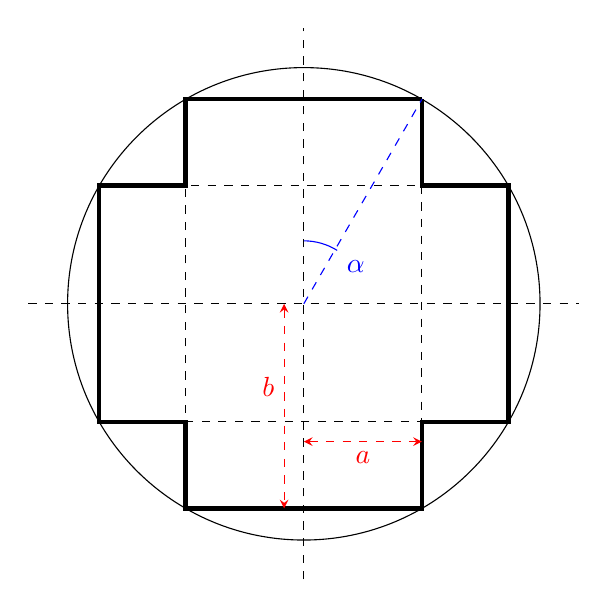
\begin{tikzpicture}
            \def\r{3}
            \def\k{2}
            
            \def\a{\r/\k}

            \pgfmathsetmacro{\b}{\r*sqrt(1-(1/\k^2))};

            \draw (0,0) circle (\r);

            \draw[ultra thick] (\a, \b) -- (\a, \a) -- (\b, \a) -- (\b, -\a) -- (\a, -\a) -- (\a, -\b) -- (-\a, -\b) -- (-\a, -\a) -- (-\b, -\a) -- (-\b, \a) -- (-\a, \a) -- (-\a, \b) -- (\a, \b);

            \draw[dashed] (-\r-0.5, 0) -- (\r + 0.5, 0);
            \draw[dashed] (0,-\r-0.5) -- (0,\r + 0.5);


            \draw[dashed, blue] (0,0) -- (\a, \b);
            \draw[blue] (0, 0+0.8) arc (90:58:0.8) node[below right] {$\alpha$};

            \draw[dashed, red, stealth-stealth] (-0.25,0) -- node[above left]{$b$} (-0.25, -\b);

            \draw[dashed, red, stealth-stealth] (0,-\a-0.25) -- node[below]{$a$} (\a,-\a-0.25);

            \draw[dashed] (\a, \a) rectangle (-\a, -\a);
        \end{tikzpicture}
    \end{figure}

    Debido a la trigonometría, sabemos que:
    \begin{equation*}
        \cos \alpha = \frac{b}{R} \Longrightarrow b = R\cos \alpha
        \qquad \qquad
        \sen \alpha = \frac{a}{R} \Longrightarrow a = R\sen \alpha
    \end{equation*}

    La función $A$ que determina el área de la figura es:
        \begin{equation*}
            \begin{array}{rl}
               A:\left]0, \frac{\pi}{4} \right[ & \longrightarrow \bb{R}\\
                        \alpha & \longmapsto A(\alpha)
            \end{array}
        \end{equation*}
        \begin{multline*}
             A(\alpha) = 2\cdot 2a2b - (2a)^2 = 8ab - 4a^2 = 4(2ab - a^2) = 4(2R^2\sen \alpha \cos \alpha - R^2\sen ^2\alpha)
             =\\=
             4R^2(\sen (2\alpha) - \sen^2\alpha) \qquad \forall \alpha \in \left]0, \frac{\pi}{4} \right[
        \end{multline*}

        Para maximizar la función, hallamos los puntos críticos.
        \begin{multline*}
            A'(\alpha) = 4R^2(2\cos(2\alpha) -\sen(2\alpha)) = 0 \Longleftrightarrow 2\cos(2\alpha) = \sen(2\alpha) 
            \Longleftrightarrow \\ \Longleftrightarrow 
            2 = \tan (2\alpha) \Longleftrightarrow \alpha = \frac{1}{2} \arctan 2
        \end{multline*}

        Veamos ahora si el punto crítico es un extremo relativo.
        \begin{equation*}
            A''(\alpha) = 4R^2(-4\sen(2\alpha) - 2\cos(2\alpha)) = -8R^2(2\sen(2\alpha) + \cos(2\alpha)) <0 \; \forall \alpha \in \left]0, \frac{\pi}{4} \right[
        \end{equation*}
        Esto se da ya que el seno y coseno son positivos en el primer cuadrante. Por tanto, como la segunda derivada es negativa, entonces se trata de un máximo relativo. También se trata de un extremo absoluto ya que es una función continua definida en un intervalo, y es el único extremo relativo.

        Por tanto, los valores que maximizan el área son:
        \begin{equation*}
            b = R\cos \alpha = \cos \left( \frac{1}{2} \arctan 2 \right)
        \qquad \qquad
            a = R\sen \alpha = \sen \left( \frac{1}{2} \arctan 2 \right)
        \end{equation*}
\end{ejercicio}